\documentclass[12pt]{article}
\usepackage{latexblog}

% ============================================================
% Blog Metadata
% ============================================================
\blogtitle{Mac上的LaTeX环境搭建}
\blogdate{2020-02-06}
\blogtags{TeX, ~LaTeX入门, LaTeX, 其他}
\bloglang{zh}
\blogsummary{}

\begin{document}
\makeblogtitle

一直希望能够自如的使用TeX来进行写作，但学习曲线还是比较高的，可惜断断续续一直没有能够入门。趁着这段时间疫情严重，待在家里又不想搞学习，那不如来重头开始学习一下吧。

\section{一些相关的概念}\label{ux4e00ux4e9bux76f8ux5173ux7684ux6982ux5ff5}

TeX \(/tɛx/\) 是高德纳（Donald Ervin Knuth）教授编写的排版软件，通俗来讲就是跟Word差不多的东西，但是TeX就好像是Markdown一样，跟编程语言差不多，不是那种所见即所得的。以下是一些相关的概念：

\subsection{TeX Engine}\label{tex-engine}

TeX引擎就是实际可以运行TeX的二进制程序，主要有以下几种：

\begin{itemize}
\tightlist
\item
  Knuth的原始 TeX，只能支持plain tex格式，\texttt{tex\ \textless{}somefile\textgreater{}}这样。现在最新的版本是\href{ftp://ftp.cs.stanford.edu/pub/tex/tex14.tar.gz}{January 12, 2014发布的版本\texttt{3.14159265}}
\item
  ε-TeX: 1990s后期发布的对TeX的一组增强扩展，实际上除了原始的TeX引擎其他的引擎都已经默认支持了这些特性
\item
  pdfTeX: pdfTeX包含了PDF 和DVI格式的输出，被许多TeX的发行版用作默认的TeX引擎
\item
  XeTeX: 同样包含了ε-TeX并原生支持Unicode和OpenType
\item
  LuaTeX: 基于pdfTeX并支持Luau脚本的TeX引擎，最初被作为pdfTeX的下一代版本但事实上形成了一个独立的分支。同样，它支持ε-TeX，使用UTF8，并能够支持嵌入Lua脚本
\end{itemize}

\subsection{TeX 格式}\label{tex-ux683cux5f0f}

TeX是一个宏（macro）处理器，macro就像是编程语言中的函数一样，

\begin{Shaded}
\begin{Highlighting}[]
\FunctionTok{\textbackslash{}def\textbackslash{}foo}\NormalTok{\{bar\}}
\end{Highlighting}
\end{Shaded}

上面这个指令会将所有的\texttt{\textbackslash{}foo}替换成\texttt{bar}。基于TeX有不同的格式，实际上就是一些macro的集合，相当于提供了一些库供用户使用，主要有以下这些：

\begin{itemize}
\tightlist
\item
  Plain TeX：原始的TeX发行版包含的基本指令集
\item
  LaTeX2e: LaTeX的最新稳定版本（最新的试验版本是LaTeX3），所有的TeX程序都支持LaTeX2e
\item
  ConTex: 另一种TeX系统
\end{itemize}

\subsection{发行版}\label{ux53d1ux884cux7248}

TeX有许多种发行版，例如：

\begin{itemize}
\tightlist
\item
  \href{https://miktex.org/}{MiKTeX}: 支持Windows的一种发行版
\item
  \href{http://tug.org/texlive/}{TeX Live}: 许多Linux/Unix默认的TeX系统，也支持Windows和Mac
\item
  \href{http://tug.org/mactex/}{MacTeX}: TeXLive的Mac版本
\end{itemize}

\subsection{总结}\label{ux603bux7ed3}

借用维基百科上的词条来总结一下吧，更加一目了然各个概念之间的区别：

\begin{figure}
\centering
\pandocbounded{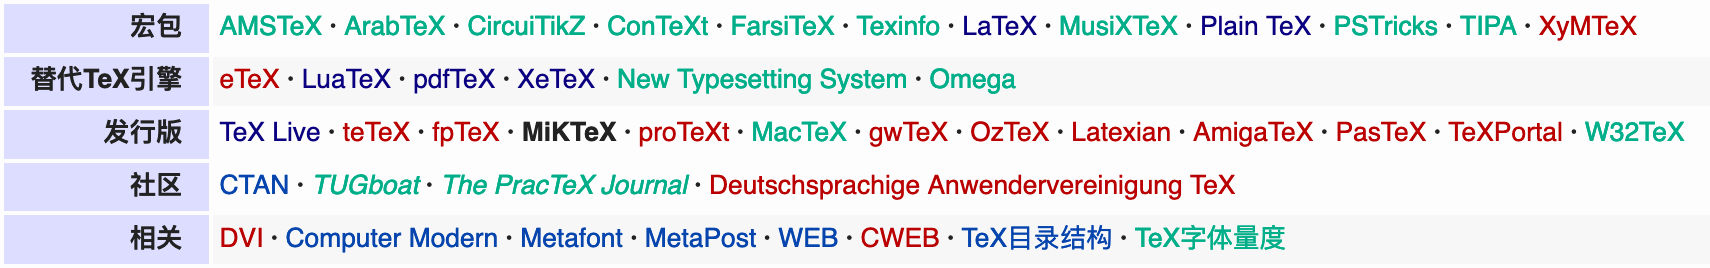
\includegraphics[keepaspectratio,alt={TeX Concepts}]{images/tex-levels.png}}
\caption{TeX Concepts}
\end{figure}

\section{Mac上的TeX环境}\label{macux4e0aux7684texux73afux5883}

Mac上推荐安装MacTeX。安装完成之后，可以看到一个TeXShop的编辑器，并可以在terminal中运行\texttt{tex}命令：

\begin{verbatim}
tex
This is TeX, Version 3.14159265 (TeX Live 2019) (preloaded format=tex)
**
\end{verbatim}

然后就是选择编辑器了，网上有不少教程，基于VSCode或者Sublime Text等的，在Mac上还有另一个选择就是Textmate了，在Textmate中安装\texttt{LaTeX}的Bundle即可，然后打开它的设置:

编写完成之后，使用Command + R运行即可预览：

值得注意的是，如果使用XeLaTeX要支持中文需要设置一下字体：

\begin{Shaded}
\begin{Highlighting}[]
\BuiltInTok{\textbackslash{}documentclass}\NormalTok{\{}\ExtensionTok{article}\NormalTok{\}}
\BuiltInTok{\textbackslash{}usepackage}\NormalTok{\{}\ExtensionTok{fontspec}\NormalTok{\}}
\FunctionTok{\textbackslash{}setmainfont}\NormalTok{\{Hiragino Sans GB\}}
\KeywordTok{\textbackslash{}begin}\NormalTok{\{}\ExtensionTok{document}\NormalTok{\}}
\NormalTok{ Hello，中国！}
\KeywordTok{\textbackslash{}end}\NormalTok{\{}\ExtensionTok{document}\NormalTok{\}}
\end{Highlighting}
\end{Shaded}

参考：

\begin{itemize}
\tightlist
\item
  \href{https://en.wikipedia.org/wiki/TeX\#cite_note-13}{TeX}
\item
  \href{https://tex.stackexchange.com/questions/49/what-is-the-difference-between-tex-and-latex}{What is the difference between TeX and LaTeX?}
\item
  \href{http://tug.org/levels.html}{LaTeX vs.~MiKTeX: The levels of TeX}
\item
  \href{https://www.latex-tutorial.com/tutorials/}{A simple guide to LaTeX - Step by Step}
\end{itemize}


\end{document}
